\chapter{慢性腹泻}

临床上如腹泻持续或反复超过4周可称为慢性腹泻,如超过6~8周则更肯定属于慢性腹泻。引起慢性腹泻的病因很多,最常见的是消化系统疾病特别是肠道本身的疾病,但全身性疾病也可以引起慢性腹泻。病因可为器质性,也可为功能性。慢性腹泻的病因学调查在国内较少报道,20世纪80年代湖南医学院一组433例住院病例报道中,以结肠癌占首位,慢性阿米巴痢疾第二位,慢性血吸虫病及肠结核又次之。此组约1/3病例为结肠癌,另1/3为各种病原体感染。但是,近年国内的一些调查显示,这一慢性腹泻的病因构成比发生了明显的变化,结肠癌仍居首位,感染性腹泻的比例逐步下降,非感染性腹泻如溃疡性结肠炎、克罗恩病、肠易激综合征、吸收不良综合征等所占的比例逐渐增加,这可能与我国现代化进程中发生的环境卫生改善及饮食习惯改变、患者的就医能力和医院的医疗水平提高等因素有关。慢性腹泻的病因分类见表\ref{tab24-1}。

\begin{longtable}{c}
 \caption{慢性腹泻疾病的分类}
 \label{tab24-1}
 \endfirsthead
 \caption[]{慢性腹泻疾病的分类}
 \endhead
 
\includegraphics[width=\textwidth,height=\textheight,keepaspectratio]{./images/Image00133.jpg}\\
 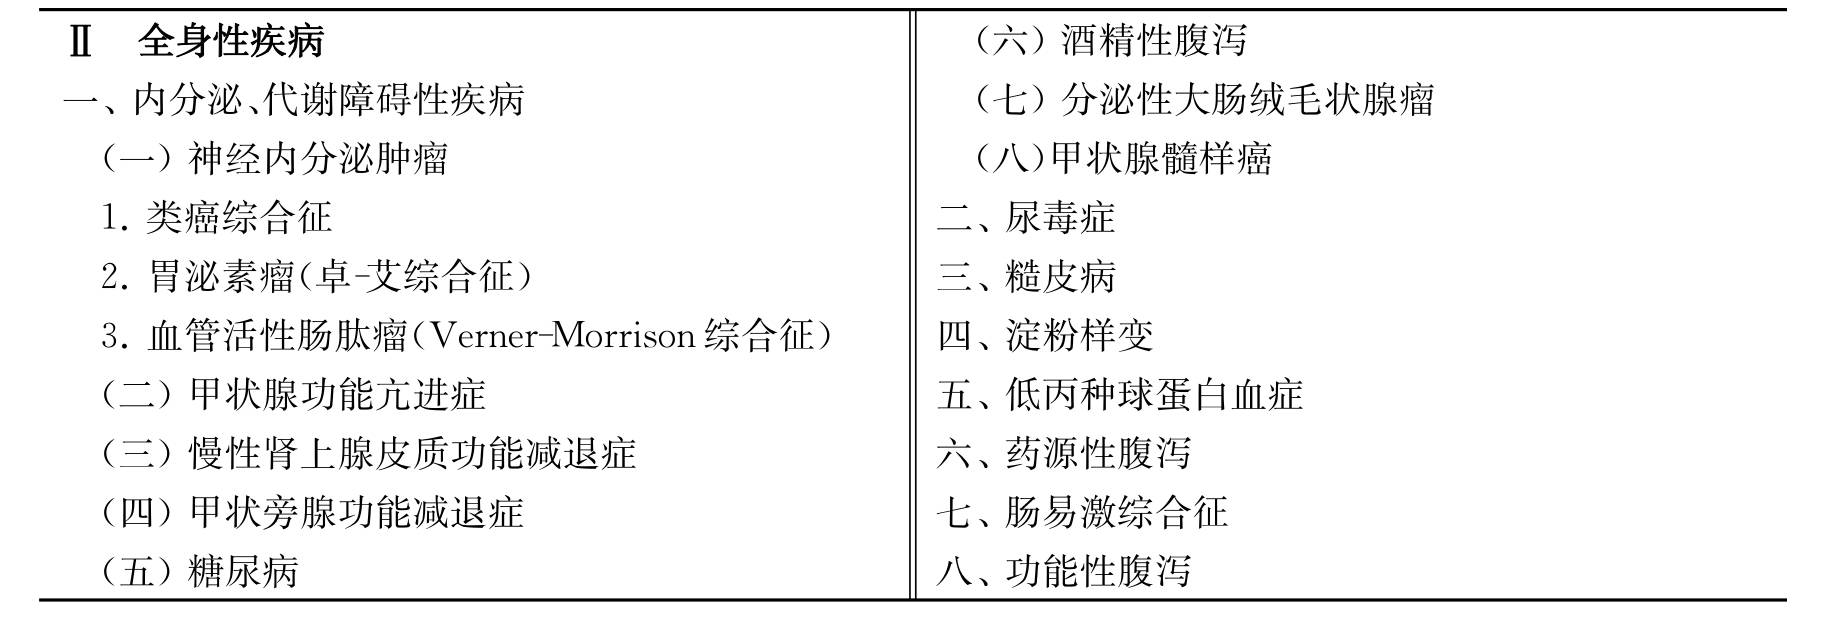
\includegraphics[width=\textwidth,height=\textheight,keepaspectratio]{./images/Image00134.jpg}
 \end{longtable}

\section{【慢性腹泻的诊断步骤】}

慢性腹泻的诊断以病史和体格检查为基础,粪便检查(包括病原体检查)作为常规(可结合血常规及一般生化检查)。诊断未明确时进行结肠镜检查和(或)X线钡剂造影检查。如仍不明确者则视不同情况进行一些特殊检查以求确诊。当高度怀疑一些有特效疗法的疾病如肠结核、阿米巴肠病等而各种检查无法确诊,最后可进行诊断性治疗试验。

\subsection{(一)病史和体格检查}

重点注意以下方面:

\subsubsection{1.病史和一般资料重点注意}

①年龄、性别;②接触史、服药史、手术史、家族史和既往病史等;③起病情况、演变过程、患病期限。

\subsubsection{2.排便情况}

\paragraph{(1)排便规律:}

注意排便次数、发生时间、诱发因素。如每天排便十多次甚至数十次,量大和水样的粪便常为分泌性腹泻;排便频繁,但量小甚至只排脓血,常提示结肠的炎症或肿瘤。半夜或清早被便意扰醒者多属器质性疾病,而肠道易激综合征多在起床或餐后排便。腹泻与便秘交替常见于肠结核、肠易激综合征、糖尿病自主神经病变者,亦见于结肠憩室炎、结肠癌。禁食可止泻的常见于渗透性腹泻,如进食麦类食物加重见于乳糜泻,进食牛乳发生者可能为乳糖不耐受症。进食某些食物或使用某些药物诱发者见于变态反应性腹泻。禁食后腹泻仍严重者,见于分泌性腹泻。

\paragraph{(2)粪便的量和性质:}

粪便量以分泌性腹泻最大,每天达数升至数十升,小肠炎症和渗透性腹泻次之,结肠炎症量最少,每次甚至只排小量脓血而不含粪质。

粪便性质的改变:如分泌性腹泻为水样便,几如清水;小肠病变为稀烂液体粪;吸收不良综合征时,酸臭糊状便见于糖吸收不良,有油滴糊状便见于脂肪吸收不良,恶臭大便见于蛋白质吸收不良。结肠病变粪便常是糊状甚至成形,炎症时粪便常带脓血,肿瘤可有血便,肠易激综合征时可有大量黏液但无脓血。

\paragraph{(3)腹痛和腹块:}

腹痛轻微或缺如常见于分泌性腹泻;腹痛突出的以炎症性腹泻多见。小肠病变的疼痛和压痛位于脐周或右下腹(回肠病变);左下腹痛多见于结肠病变,直肠受累则多有里急后重。

腹块常是肿瘤或炎症性病变,其部位和性质可提示受累肠段和病变性质。肛门指检应列为常规,在粪便带血时特别重要,约50\%大肠癌发生在直肠,可被指检发现。

\paragraph{(4)其他伴随的腹部及全身症状和体征:}

发热、贫血、消瘦、肝脾大、肛周脓肿和瘘管,与腹泻有关的一些肠外表现如口腔溃疡、关节炎、皮疹等,对鉴别诊断大有帮助。此外,不要忽略非腹部疾患所引起的腹泻,并注意作相应检查。

\subsection{(二)实验室检查}

1.粪便检查

\subsubsection{(1)粪便常规检查:}

医师宜亲自观察患者所排的新鲜粪便,肉眼检查其量及性状已如前述。粪便常规检查包括隐血试验及显微镜检查红白细胞、原虫、虫卵、脂肪滴。

\subsubsection{(2)粪便培养:}

可发现致病菌,对感染性腹泻诊断尤为重要。

值得指出的是,慢性腹泻的病原体有时不易找到,如有怀疑,应作多次检查。如能视情况采取进一步检测手段,如血吸虫卵孵化、阿米巴或血吸虫的血清学检查、肠道厌氧菌培养、真菌培养等,可望有更多“未明原因”腹泻得到病原学的确诊。

2.血常规和生化检查可了解有无贫血、白细胞增多和糖尿病、尿毒症等,以及了解水、电解质和酸碱平衡情况。

3.怀疑肠结核要行PPD皮试和干扰素-γ释放试验(T-SPOT-TB)。疑及风湿性疾病相关的肠道病变时行自身免疫抗体的有关检查。

\subsection{(三)结肠镜、小肠内镜和放射影像学检查}

\subsubsection{1.结肠镜检查}

结肠镜检查是慢性腹泻鉴别诊断最常用的检查,检查时宜进入回肠末段。通过直接观察结直肠和回肠末段黏膜并结合活检以助诊断。

\subsubsection{2.胶囊内镜或(及)气囊辅助小肠镜}

有助于发现小肠病变。胶囊内镜对小肠病变的检出率高,但因不能活检,常不能定性。对发现小肠病变而不能定性者或虽无发现而高度怀疑小肠病变者可行气囊辅助小肠镜检查。

\subsubsection{3.CT小肠成像(CTE)或MR小肠成像(MRE)}

对显示小肠炎性病变有特殊价值,目前已成为炎症性肠病诊断和鉴别诊断的常规检查。

\subsubsection{4.X线钡餐或(和)钡剂灌肠造影}

可观察全胃肠道的功能状态、有无器质性病变,但敏感性低,有条件的医疗机构多以内镜或CTE/MRE取代之。

\subsection{(四)特殊检查}

\subsubsection{1.吸收功能检查}

各种不同的吸收功能检查用于吸收不良综合征的不同疾病的诊断。这些检查包括粪脂测定、D-木糖吸收试验、胰外分泌功能试验、\textsuperscript{75}
Se-牛黄胆酸潴留试验、葡萄糖或乳糖氢呼气试验等。

\subsubsection{2.血浆激素和介质测定}

铬粒素A(chromogranin
A,CgA)是目前公认最有价值的胃肠胰神经内分泌肿瘤通用肿瘤标志物,血清或血浆CgA升高诊断胃肠胰神经内分泌肿瘤的敏感度和特异度在70\%~100\%。对特定的有功能的胃肠胰神经内分泌肿瘤,测定其分泌的激素或介质有确诊价值,如促胃液素(胃泌素瘤)、5-羟色胺(类癌)、血管活性肠肽(VIP瘤)等。此外,血清甲状腺素测定对甲状腺功能亢进引起的腹泻有诊断价值,降钙素对甲状腺髓样瘤引起的腹泻有参考价值。

\subsubsection{3.B超和CT}

可了解肝、胆、胰等内脏病变。必要时还可辅以超声内镜检查。

\subsubsection{4.磁共振胰胆管成像(MRCP)或逆行胰胆管造影(ERCP)}

疑为胆道或胰腺疾病引起的腹泻,必要时可作ERCP或MRCP检查。

\section{【慢性腹泻的诊断思路】}

慢性腹泻的病因相当广泛,有时颇为复杂,其病因的诊断与鉴别诊断首先从临床病史及体检资料入手,以排便情况和粪便检查作为起点,推测腹泻发病机制分类以及腹泻来源于小肠还是大肠,然后按步骤、有重点地进行检查,最终找出病因。

\subsection{(一)功能性腹泻与器质性腹泻的鉴别}

门诊所见的慢性腹泻病例有相当部分为功能性腹泻(最常见为肠易激综合征),临床上有可能根据详细的病史询问和细致的体格检查将这部分功能性腹泻的病例与器质性腹泻作出初步的区分,从而尽快作出诊断,以减轻患者的痛苦和医疗费用。一般而言,年轻患者(<40岁)、病史长(>1年)而症状常为间歇性,一般状况良好而无体重下降,大便次数增加而总量增加不明显,粪便可带黏液而绝无脓血,多于早晨或餐后排便而无半夜或清早为便意扰醒,则可考虑多为功能性。如大便常规检查阴性,可作出初步临床诊断,必要时进行结肠镜检查则诊断基本确立。对于半夜或清早为便意扰醒,体重下降,腹部压痛明显或有包块,粪便带血或大便常规检查隐血试验阳性者,提示器质性腹泻,应进行彻底检查查明病因。对年龄在40岁或以上的慢性腹泻患者,宜常规结肠镜检查以免漏诊结肠癌。

\subsection{(二)按发病机制进行的腹泻分类}

1.渗透性腹泻是由于肠腔内含有大量不能被吸收的溶质,使肠腔内渗透压升高,大量液体被动进入肠腔而引起腹泻。引起渗透性腹泻的病因可分成两大类:一类是服食不能吸收的溶质,包括某些泻药和其他一些药物,如硫酸镁、乙二醇聚乙烯(PEG)、甘露醇、山梨醇、乳果糖等。另一大类为小肠对糖类吸收不良,见于各种疾病引起的吸收不良综合征[消化和(或)吸收功能障碍]。其中一些疾病是由单一的糖吸收不良所导致的渗透性腹泻,在我国以成人乳糖酶缺乏最为常见。另一些疾病除因糖吸收不良导致渗透性腹泻外,尚伴有脂肪和蛋白吸收不良,临床表现为脂肪泻(粪便含有大量脂肪,呈大容量、腐臭味、浅黄或灰白色稀水样便或糊状便,表面常漂浮油脂层),常伴有多种物质吸收障碍所致的营养不良综合征。渗透性腹泻在临床上的主要特点是禁食后腹泻停止或显著减轻,与脂肪消化、吸收不良有关的疾病有脂肪泻。

2.分泌性腹泻是由于肠黏膜上皮细胞电解质转运机制障碍,导致胃肠道水和电解质分泌过多或(及)吸收受抑制而引起的腹泻。典型的单纯性分泌性腹泻见于具有分泌促分泌物功能的肿瘤如类癌、胃泌素瘤、血管活性肠肽瘤、甲状腺髓样癌和分泌性直肠或结肠绒毛状腺瘤等。这类腹泻的临床特点是大量水样便,禁食后腹泻不减轻。

3.炎症性腹泻是由于肠黏膜的炎症、糜烂和溃疡等病变导致炎性渗出物进入肠腔。此时炎症渗出虽占重要地位,但因肠壁组织炎症而导致肠分泌增加、吸收不良和运动加速等病理生理过程在腹泻发病中亦起很大作用。炎症性腹泻是最常见的慢性腹泻,可分为感染性和非感染性两大类。前者包括细菌、病毒、寄生虫、真菌感染等;后者包括免疫因素、肿瘤、物理化学因素及血管性疾病等引起的肠道炎症病变。这类腹泻的特点是粪便含有渗出液和血。结肠特别是左半结肠病变多有肉眼脓血便:小肠病变渗出物及血均匀地与粪便混在一起,除非有大量渗出或蠕动过快,一般无肉眼脓血,需依靠隐血试验和显微镜检查发现。

4.运动功能异常性腹泻是由于肠蠕动加快,以致肠腔内水和电解质与肠黏膜接触时间缩短,而影响水分吸收,导致腹泻。肠腔内容量增加可引起反射性肠蠕动加快,因此上述3种类型的腹泻发病中亦必然有肠运动功能异常的机制参与。临床上,在腹泻发病机制中肠运动功能增加起主要作用的腹泻主要见于肠易激综合征。某些全身性疾病通过神经体液的因素可引起肠功能紊乱性腹泻,如甲状腺功能亢进、糖尿病性神经病、肾上腺皮质功能减退症等。单纯肠运动功能异常性腹泻的特点是粪便不带渗出物和血,一般表现为大便次数增加而大便总量增加不明显。

临床上根据排便的特点,如是否为大量水样便、是否有脂肪泻、禁食后腹泻是否可减轻、粪便中是否有肉眼或显微镜下脓血便(包括隐血试验)等,有可能大致推测慢性腹泻的发病机制分类,从而缩窄需要鉴别的病因的范围。应当指出,不少腹泻并非由某种单一机制引起,而是多种因素共同作用下发生的,因此对一些复杂病例需要更细致的分析和更深入的检查。

\subsection{(三)大肠性腹泻与小肠性腹泻的鉴别}

可以根据临床表现的特点粗略估计引起腹泻的病变部位可能在大肠还是小肠(表\ref{tab24-2})。结肠镜检查可以肯定或排除大肠的病变,因此对疑为器质性腹泻的患者结肠镜可作为首选检查。

\begin{table}[htbp]
\centering
\caption{小肠性腹泻与结肠性腹泻的鉴别要点}
\label{tab24-2}
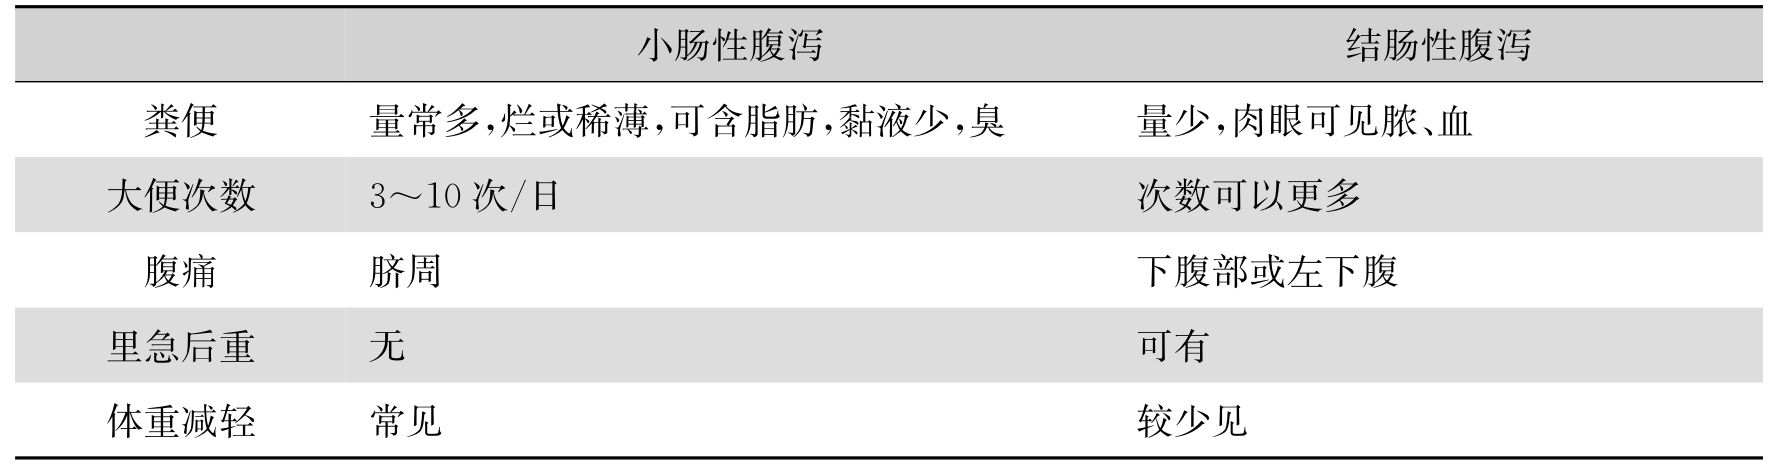
\includegraphics[width=5.9375in,height=1.57292in]{./images/Image00135.jpg}
\end{table}

根据临床表现及粪便检查,按照上述思路,一般可以初步估计慢性腹泻病因的可能范围,对肠易激综合征或某些具有流行病学特征的感染性腹泻(如慢性阿米巴痢疾、慢性细菌性痢疾和慢性血吸虫病等)则多可作出临床诊断。再进行结肠镜检查,大部分慢性腹泻病例可获病因诊断。小部分病情复杂而诊断有困难的病例,可根据估计的病因范围,选择相应的检查,逐步深入,则绝大部分慢性腹泻病例可获病因诊断。

\protect\hypertarget{text00190.html}{}{}

\section{76 消化系疾病}

\subsection{76.1 肠道疾病}

\subsubsection{76.1.1 慢性肠道感染性疾病}

\paragraph{一、慢性细菌性痢疾}

慢性细菌性痢疾是由于急性细菌性痢疾治疗不当演变而成。慢性菌痢可区分为下列三型:①慢性隐匿型:患者过去有急性菌痢史,已隔两个月以上无症状,但结肠镜检有病理改变或同时大便培养痢疾杆菌阳性。②慢性迁延型:急性菌痢病情长期迁延不愈。患者有不同程度的腹部症状,如腹痛、腹胀、腹泻,或腹泻与便秘交替出现。大便间歇地或经常地带有黏液或脓血。大便间歇排菌,培养有时阳性,有时阴性。③慢性型急性发作:患者在慢性过程中,因某种原因(如受凉、饮食失调)的激惹而急性发作,腹痛与腹泻加重,便脓血,里急后重,可伴有发热,临床表现与急性菌痢相似。

慢性菌痢的诊断主要根据过去急性病史及大便检查的阳性结果。大便外观多为黏液性或脓血样,也有只呈糊样或水样,但镜检仍可发现白细胞。大便培养有特别重要的诊断价值。在结肠镜直视下,从病灶直接采取标本进行培养,会获得较高的阳性率。多次反复的大便培养(一般须连续三次)或在急性发作时进行培养,可提高阳性率。标本愈新鲜愈好。慢性细菌性痢疾大便培养阳性率比急性期明显下降,因而较易漏诊。对慢性腹泻特别是有急性痢疾样发作史,结肠镜检查显示慢性结肠炎的患者,不要轻易下“慢性结肠炎”的诊断,应进行多次大便培养,积极寻找病因。

慢性细菌性痢疾须与慢性阿米巴痢疾鉴别。慢性阿米巴痢疾主要根据大便镜检发现溶组织阿米巴或(及)抗阿米巴治疗的疗效而确定。近年研究发现,部分急性菌痢患者经治愈后,仍会有慢性腹泻症状,但经严格的细菌学检查证实已无痢疾杆菌感染,结肠镜检查亦无肉眼及组织学的病变,此种情况称为感染后肠易激综合征,要注意与慢性细菌性痢疾鉴别。

\paragraph{二、肠 结 核}

肠结核近年已较少见,但绝非罕见。多数患者同时有开放性肺结核,但亦有患者肺结核已痊愈或肺结核病史不明确。本病好发于中青年。临床表现为腹泻、腹痛、右下腹压痛,可有腹块。多伴有发热、盗汗等结核毒血症状。就诊时病程多较长,故体重下降常见。本病腹泻一般每日2~4次,粪便呈糊样,一般无肉眼脓血便,但大便常规检查隐血试验多呈阳性。有些患者会出现腹泻与便秘交替,这与病变引起的胃肠功能紊乱有关。肠结肠病变好发于回盲部,结肠镜检查发现主要位于回盲部(回肠末段、回盲瓣、盲肠升结肠)的肠黏膜炎症、溃疡、炎症息肉或肠腔狭窄,结合活检如见干酪样坏死性肉芽肿具确诊意义(但阳性率不高),活检抗酸杆菌染色阳性有助诊断,活检组织结核杆菌聚合酶链反应(TB-PCR)阳性有助诊断。同时行小肠放射影像学检查(CT小肠成像或X线小肠钡剂检查)见病变只局限在回肠末段亦有助诊断。PPD皮肤试验强阳性有助诊断,干扰素-γ释放试验(T-SPOT-TB)阴性倾向于排除结核。对中青年患者特别是伴有肺结核,具有典型临床表现和结肠镜检查及小肠放射影像学检查所见,可高度怀疑肠结核;如抗结核治疗(2~4周)症状明显改善,并于2~3个月后肠镜复查病变痊愈或明显好转,可作出肠结核的临床诊断;继续完成正规抗结核疗程,疾病痊愈无复发为临床确诊。对有手术指征者行手术探查,病变肠段或(及)肠系膜淋巴结病理组织学检查发现干酪样坏死性肉芽肿可确诊。

本病主要与克罗恩病鉴别,但有时两者鉴别十分困难。两病的鉴别要点参见第76.1.2节克罗恩病的相关内容。肠结核有时还要注意与小肠恶性淋巴瘤以及艾滋病合并肠道感染等疾病鉴别。

\paragraph{三、慢性阿米巴痢疾}

阿米巴痢疾发病缓渐,为慢性经过,有复发的倾向。病变较常侵及盲肠与右侧结肠,乙状结肠与降结肠次之。即使在急性发作期,患者的发热、排便次数、里急后重与腹痛的程度也不及细菌性痢疾。细菌性痢疾时,腹部压痛常以左下腹部较著,而阿米巴痢疾时,压痛常以右下腹部较著。两者的大便性状也有所不同,细菌性痢疾常为脓血便或鲜红色的黏液血便,无特别的恶臭;阿米巴痢疾大便色常暗红,有如果酱,如含有崩溃腐败的组织,大便常有特别的恶臭。也应指出,病例中粪便呈糊状而无上述情况者也不少。

阿米巴痢疾的诊断须根据大便镜检发现溶组织阿米巴滋养体或其包囊。在粪便检查应挑选含血、黏液部分,标本应尽快进行检查(新鲜大便),阴性结果时要反复多次检查,采用浓缩法可提高阳性率。如仍为阴性结果,可行结肠镜检查,镜下可见结肠黏膜散在分布的潜行溃疡,溃疡间黏膜正常,在溃疡边缘涂片及活检可见滋养体。如患者临床表现符合阿米巴痢疾,虽大便检查阴性,而抗阿米巴药物治疗有效,也可诊断为此病。此病与慢性菌痢及其他病因慢性结肠炎的鉴别,主要依靠病原体的检出及抗阿米巴疗效佳。

\paragraph{四、慢性血吸虫病}

慢性血吸虫病虫卵沉积于肠壁的黏膜和黏膜下层,反复感染和成虫产卵可导致肠壁炎症改变和纤维化。慢性血吸虫病由肠道炎症引起的慢性腹泻,多为每日2~3次,间或便中带黏液与血,也可呈腹泻便秘交替。可伴有腹痛。晚期患者可扪及左下腹包块或痉挛性条索状物(乙状结肠肉芽肿形成或纤维化)。肠镜下活动性炎性病变表现为黏膜红肿、糜烂和溃疡;慢性病变表现为颗粒状、结节状、息肉状或肿块状,病变形态缺乏特异性,活动性炎症可与慢性病变共存于同一部位或不同肠段。病变分布部位不一,但以乙状结肠和直肠最为明显。确诊依据找到血吸虫卵,粪便常规检查可检出血吸虫卵,病变黏膜活检或直肠黏膜活检压片显微镜下更易检出虫卵。

晚期血吸虫病也可引起小肠吸收不良,原因可能由于胰腺外分泌功能减退、门脉高压、肠系膜淋巴循环障碍或阻塞所致。

\paragraph{五、肠鞭毛虫病}

\subparagraph{(一)贾第虫病}

又称梨形鞭毛虫病,是蓝伯贾第虫寄生于小肠所致的疾病。患者一般因腹泻稀便而就诊,1/3病例有轻度腹痛,部分有固定的疼痛部位,可位于腹部任何区域。病程长,个别病例达30年。此虫所引起的腹泻一般较轻,大多为稀便或稀水便,往往被忽视而未及时诊断与治疗,尤以小儿为然。误诊为慢性菌痢或慢性阿米巴痢者也有之。急性菌痢或急性阿米巴痢同时合并此虫感染,若不同时进行治疗,大多遗留慢性腹泻而不易治愈。大便涂片镜检见贾第虫滋养体而确诊,大便中通常只有少数脓细胞与红细胞。甲硝唑治疗有特效。此虫引起胆道感染者国内也有报告。

\subparagraph{(二)迈氏唇鞭毛虫病}

迈氏唇鞭毛虫病和人肠滴虫病都有极高的传染性与致病性,据国内一组病例报告,腹泻、腹痛、腹胀等症状都很顽固。人肠滴虫病国内报告多急性起病,并反复发作,且经久不愈,有时甚至和肠阿米巴病、菌痢难以区别。大便镜检发现此虫而确诊。甲硝唑治疗有效。

\paragraph{六、结肠小袋纤毛虫病}

本病皆因与病猪接触而致感染,主要表现为腹痛与稀便,每天数次,带黏液,可混有血液,类似轻型菌痢,大便镜检找到此虫而确诊。结肠镜检可见黏膜小溃疡,多呈圆形或椭圆形,常被覆一层不牢固的白色假膜,拭去假膜即见基底充血与出血。此种假膜为本病所特有,有别于菌痢与阿米巴痢疾。在结肠镜检前不宜清洁灌肠,以免假膜剥落而难于发现。从假膜刮出的黏液作涂片检查,易找到此虫。

\paragraph{七、肠道蠕虫病}

重度的钩虫、姜片虫、绦虫、鞭虫、粪类圆线虫等感染,均可引起慢性腹泻、便溏,或伴有腹痛,大便镜检易找到虫卵或幼虫。

\paragraph{八、艾滋病合并肠道感染}

艾滋病临床C型即AIDS期合并肠道机会感染而表现为慢性腹泻,是艾滋病的常见症状。肠道感染的病原体有原虫(常见如隐孢子虫)、病毒(常见如巨细胞病毒、单纯疱疹病毒)、真菌(常见如白念珠菌)、细菌(鸟型分枝杆菌、沙门菌、弯曲菌属)等。病变可在小肠或(及)大肠,腹泻可表现为炎症性腹泻或(及)脂肪泻,结肠镜及X线胃肠钡餐检查可见各种病变表现。随着我国艾滋病的不断增加,艾滋病合并肠道感染在我国已有不少报道,诊断的关键是提高对艾滋病的警惕和认识,遇有难以解释的慢性腹泻,特别是伴有不明原因发热、消瘦的患者,要想到艾滋病的可能,询问接触史并及时进行HIV病原学检测。

\subsubsection{76.1.2 炎症性肠病}

目前,临床上普遍使用炎症性肠病(inflammatory bowel
disease,IBD)这一名称来表示溃疡性结肠炎和克罗恩病(Crohn病)。此外,这一概念也包括那些难于区分是溃疡性结肠炎还是克罗恩病的结肠炎,即未确定型结肠炎(indeterminate
colitis)。这类疾病发病率有明显的地域差异及种族差异,以北美、北欧白种人最高,亚洲黄种人较低。我国近年发病有明显增加趋势,其中以溃疡性结肠炎较多见。发病高峰年龄为20~40岁,亦可见于儿童或老年。

\paragraph{一、溃疡性结肠炎}

本病为直肠和结肠的慢性非特异性炎症,病变主要局限在黏膜层,呈从肛端直肠开始向近端扩展的连续性、弥漫性分布。

起病多数缓慢,少数急性起病,偶见急性暴发起病。病程呈慢性经过,多表现为发作期与缓解期交替。腹泻和便血是本病最常见和最突出的症状。大便次数及便血的程度反映病情活动性的轻重。病变限于直肠或直肠乙状结肠患者,除可有便频、便血外,偶尔反有便秘,这是病变引起直肠排空功能障碍所致。常伴腹痛,一般为轻度至中度,多为左下腹或下腹的阵痛。常有里急后重。中、重型患者活动期常有低度至中度发热,重症或病情持续活动可出现衰弱、消瘦、贫血、低蛋白血症等表现。本病可伴有多种肠外表现,包括关节、皮肤、口腔、眼等。

结肠镜检查是本病诊断与鉴别诊断的最重要手段。应作全结肠及回肠末段检查,直接观察肠黏膜变化,取活组织检查,并确定病变范围。本病病变呈连续性、弥漫性分布,从肛端直肠开始逆行向近端扩展,内镜下所见重要改变有:①黏膜粗糙呈细颗粒状,弥漫性充血、水肿,血管纹理模糊,质脆、出血,可附有脓性分泌物。②病变明显处见弥漫性糜烂或多发性浅溃疡。③慢性病变见假息肉及桥状黏膜,结肠袋往往变钝或消失。结肠镜下黏膜活检组织学见弥漫性炎症细胞浸润,活动期表现为表面糜烂、溃疡、隐窝炎、隐窝脓肿;慢性期表现为隐窝结构紊乱、杯状细胞减少。

X线钡剂灌肠检查所见X线征主要有:①黏膜粗乱及(或)颗粒样改变;②多发性浅溃疡,可有炎症性息肉;③肠管缩短、结肠袋消失呈铅管状。因结肠镜检查比X线钡剂灌肠检查准确,有条件宜作结肠镜全结肠检查,检查有困难时才辅以钡剂灌肠检查(重型或暴发型病例不宜作钡剂灌肠检查,以免加重病情或诱发中毒性巨结肠)。

溃疡性结肠炎的临床诊断主要基于临床表现、结肠镜检查和活检。具有持续或反复发作腹泻和黏液脓血便,在排除细菌性痢疾、阿米巴痢疾、慢性血吸虫病、肠结核等感染性肠炎及克罗恩病、缺血性肠炎、放射性肠炎等非感染性肠炎基础上,具有上述结肠镜检查重要改变中至少1项及黏膜活检组织学所见可以诊断本病。初发病例如临床表现、结肠镜及活检改变不典型者,可列为“疑诊”随访。应强调,本病肠镜所见及活检组织学所见虽有一定特点但均非特异性改变,各种病因均可引起类似的肠道炎症改变,故只有在认真排除各种可能有关的病因后才能作出本病诊断。其中,大便的病原学检查对感染性肠炎的鉴别至关重要,须反复进行。本病与病变局限在结肠的克罗恩病的鉴别详见下文克罗恩病。

\paragraph{二、克罗恩病}

本病是一种胃肠道的慢性炎性肉芽肿性疾病。与溃疡性结肠炎不同,其病变可累及全消化道,但以同时累及回肠末段与邻近结肠者为最多见,也可只累及小肠或局限在结肠。病变呈非连续性(节段性或跳跃性)分布,多累及肠壁全层。

起病隐匿、缓渐,慢性病程多呈活动期与缓解期交替。临床主要表现为腹痛、腹泻和体重下降。常伴发热等全身症状。病情发展可出现肠梗阻、瘘管、腹腔脓肿等并发症。可有肛周病变。可伴有多种肠外表现,包括关节、皮肤、口腔、眼等。本病腹泻程度轻重不一,但大多无肉眼血便及里急后重(累及肛门直肠者除外)。

结肠镜是诊断克罗恩病的首选检查方法。结肠镜作全结肠及回肠末段检查。病变呈节段性(非连续性)分布,纵行溃疡和卵石样外观是克罗恩病的主要特征,但不是每例都有此类典型病变。多部位多块活检见非干酪坏死性肉芽肿有助诊断。应同时行小肠检查,因为克罗恩病的病变可以只局限在小肠,再者,如发现小肠和结肠同时存在多处节段性病变有利于克罗恩病的诊断。小肠检查以CTE/MRE最常用,必要时辅以胶囊内镜或(及)气囊辅助小肠镜。

克罗恩病的临床诊断需要结合临床、内镜、放射影像学检查及活检进行综合分析。对治疗反应的随访(一般1年以上)有助确诊。手术切除肠段以及肠系膜淋巴结的病理大体及组织学检查见克罗恩病典型表现可确立诊断,适用于有手术指征的患者。作出临床诊断之前必须排除各种肠道感染性或非感染性炎症疾病及肠道肿瘤。

病变局限在结肠的结肠型克罗恩病须与溃疡性结肠炎鉴别,鉴别要点是:①溃疡性结肠炎病变从肛端直肠开始逆行向近端扩展,病变呈连续性和弥漫性,极少数病例可见回肠末段数厘米内黏膜炎症改变但无溃疡形成。如见直肠不受累的结肠病变、病变肠段间有正常黏膜的肠段(非连续性)、纵行溃疡间有正常黏膜(非弥漫性)则为克罗恩病特征。②复杂的肛周病变、瘘和腹腔脓肿仅见于克罗恩病。③肠腔明显狭窄多见于克罗恩病。④活检如见非干酪性肉芽肿支持克罗恩病诊断。然而,即使仔细鉴别,仍有少部分(西方文献报道约10\%)结肠IBD无论结肠镜及活检组织学所见仍无法肯定分类,对上消化道及小肠进行仔细检查亦未发现病变,此时临床可诊断为IBD类型待定(inflammatory
bowel disease unclassified,IBDU)。而未定型结肠炎(indeterminate
colitis,IC)指结肠切除术后病理检查同时具备克罗恩病及溃疡性结肠炎病理特征者。

在我国,克罗恩病与肠结核的鉴别尤为重要。肠结核与回结肠型克罗恩病鉴别常会相当困难,因为除活检发现干酪样坏死性肉芽肿为肠结核诊断的特异性指标外,两病在临床表现、结肠镜下所见及活检所见常无特征性区别,然干酪样坏死性肉芽肿在活检中的检出率却很低(不超过1/3)。因此强调,在活检未见干酪样坏死性肉芽肿情况下,鉴别依靠对临床表现、结肠镜下所见及活检进行综合分析。下列表现倾向克罗恩病诊断:肛周病变(尤其是肛瘘/肛周脓肿),疑为克罗恩病的肠外表现如反复发作口腔溃疡、皮肤结节性红斑等,并发瘘管、腹腔脓肿;结肠镜下见典型的纵行溃疡、典型的卵石样外观、病变累及≥4个肠段、病变累及直肠。TSPOT阴性有利排除肠结核而倾向克罗恩病诊断。下列表现倾向肠结核诊断:伴活动性肺结核,结核菌素试验强阳性;结肠镜下见典型的环形溃疡、回盲瓣口固定开放;活检见肉芽肿数目多、直径大(长径>400μm)、特别是有融合,抗酸染色阳性,TB-PCR阳性。小肠检查对两病鉴别有帮助,如回结肠病变与近段小肠(末段回肠以近)病变,特别是多节段病变共存,倾向克罗恩病诊断。鉴别仍有困难者,予诊断性抗结核治疗,治疗数周内(2~4周)症状明显改善,并于2~3个月后肠镜复查病变痊愈或明显好转,可作出肠结核的临床诊断。有手术指征者行手术探查,绝大多数肠结核可在病变肠段或(及)肠系膜淋巴结病理组织学检查中发现干酪样坏死性肉芽肿而获确诊。

\subsubsection{76.1.3 其他原因的肠炎}

\paragraph{一、缺血性结肠炎}

缺血性结肠炎是缺血性肠病(参见第71节)中最常见的一种类型,专指由结肠缺血所致的结肠病变。以老年人常见,但亦可见于年轻人。一般认为其发病是由结肠局部缺血及再灌流损伤所致。多为一过性的局部血管缺血而难以找到明确病因及血管解剖学的阻塞或狭窄。能发现明确病因者,如肠系膜动脉血栓形成或栓塞、脓毒血症、失血性休克、心力衰竭、结肠扭转等,则往往预后不佳。一些可能与发病有关的危险因素包括:血管炎和一些先天性或获得性凝血障碍疾病、各种药物如可卡因、止泻药、泻药、雌激素、非甾体消炎药、血管收缩剂等、巨细胞病毒或大肠杆菌O157∶H7感染;一些疾病状态如肠易激综合征、主动脉或冠脉手术、结肠机械梗阻等;长跑运动。病变可累及全大肠任何部位,呈节段性分布。原本血供较差而当发生缺血时侧支循环较难迅速建立的区域为好发部位,如乙状结肠或降结肠;单独累及直肠者少见;单独累及右半结肠者病情凶险,此常为肠系膜上动脉阻塞所致的急性肠系膜缺血的警报,常同时或继而累及小肠(又称“缺血性小肠结肠炎”)。

临床上多急性起病,表现为突然发作的左侧腹痛及便意,24小时内出现腹泻、血便。体检在病变累及肠段部位有轻至中度压痛。腹痛程度多为轻至中度,便血量一般未到需要紧急输血的程度。病程多呈自限性,可于数天内症状消失。如症状持续超过2周者,多提示存在慢性或进展性病变,可发展为瘢痕狭窄及至肠梗阻。“坏疽型缺血性结肠炎”少见但病情重,可并发坏疽和穿孔;呈暴发者罕见,可并发中毒性巨结肠。腹部平片可作为初筛检查,可见指压征。结肠镜检查是诊断该病的重要手段,具确诊意义。应尽早于起病48小时内完成检查,因为之后典型的出血性病变会消失或改变。本病内镜下病变呈节段性分布且病变肠段与正常肠段界限清楚,极少累及直肠。典型者病变具有3个演变期:①急性期,在起病48小时内,镜下可见黏膜充血、水肿、黏膜下出血,此期典型病变为出血性结节(相当于X线所见的指压征)。②亚急性期,起病数天至2周内,复查内镜见糜烂,或深或浅的溃疡,可呈环周或呈单条纵行,可见坏死渗出物或假息肉等改变;亦可见病变完全消失,黏膜恢复正常。③恢复期或慢性期,内镜下黏膜恢复的时间取决于病变的严重程度及演变,一般从起病1~2周至数月甚至6个月,内镜下病变逐渐改善至消失,此期症状多已消失或明显改善;少数病例可发展为纤维狭窄或慢性结肠炎。活检病理组织学特征性改变为梗死或空壳细胞;支持该病的改变为黏膜及黏膜下出血及毛细血管纤维性血栓形成伴中性粒细胞浸润。但亦常见类似IBD的改变,如隐窝脓肿、溃疡、黏膜及黏膜下纤维化等。血管造影无助诊断,因到出现症状时结肠血管已恢复正常。但下列情况除外:病变单独累及右半结肠或无法与急性肠系膜缺血鉴别,此时肠系膜血管造影的目的是及早判断有无肠系膜上动脉阻塞以便及时处理。

本病临床表现及结肠镜所见与炎症性肠病有相似之处,应注意鉴别。老年患者、临床表现为急性起病、先有腹痛继血便;48小时内内镜检查见节段性病变、出血性结节;病程呈自限性;内镜随访病变呈典型的演变过程;结合活检病理组织学所见,与IBD鉴别不难。但在病程中期就诊者常需与初发型IBD鉴别。鉴别诊断中年龄是一个重要因素,初发的IBD少见于50岁以上。缺血性结肠炎节段性分布与克罗恩病(CD)相似,如见纵行溃疡、卵石样外观,结合CD的肠外表现和肛周病变则支持CD;反之自限性临床过程及内镜下病变演变过程支持缺血性结肠炎。黏膜弥漫性充血、水肿、糜烂、溃疡,活检见隐窝脓肿与UC相似,但缺血性结肠炎呈节段分布,少见直肠受累,结合自限性临床过程及内镜下病变演变过程可作鉴别。

\paragraph{二、嗜酸性粒细胞性胃肠炎}

本病是一种较少见的胃肠疾病,以嗜酸性粒细胞(全部或为主)浸润胃肠道黏膜和黏膜下层,甚至肌层和浆膜层,但大多数情况下无腺体破坏为典型特点。本病临床表现随炎症累及肠壁层次不同而异。仅累及黏膜和黏膜下层时,表现为腹绞痛、恶心、呕吐、腹泻、体重下降;累及肌层时,表现为肠梗阻或幽门梗阻;累及浆膜层时,表现为腹水,腹水中见大量嗜酸性粒细胞。临床上以第一种情况最为常见。外周血嗜酸性粒细胞多增高,但也可在某一病期表现为正常。内镜检查结合活检是确立诊断的重要手段。病变可累及全消化道,多分布广泛而散在,但以胃及上段小肠最常见,一般先行胃镜检查,必要时再作结肠镜及小肠镜检查。内镜下所见无特异性,表现为充血、水肿、糜烂、溃疡、结节等,亦可肉眼正常,多部位(包括镜下病变部位及正常部位)活检甚为重要。本病诊断需符合下列标准:①有消化系统症状;②病理证实胃肠道一处或多处组织嗜酸性粒细胞浸润;③无胃肠道以外多器官嗜酸性粒细胞浸润,并除外引起肠道嗜酸性粒细胞浸润的其他疾病如寄生虫感染等。本病需特别注意与高嗜酸性粒细胞综合征鉴别,后者外周血嗜酸性粒细胞高达1.5×10\textsuperscript{9}
/L,有多器官嗜酸性粒细胞浸润表现。嗜酸性粒细胞肠炎对糖皮质激素治疗常有良好反应,停药后虽可反复,但一般预后良好。

\paragraph{三、显微镜下结肠炎(淋巴细胞性结肠炎和胶原性结肠炎)}

显微镜下结肠炎以非血性水样泻、结肠镜下黏膜正常或大致正常、活检病理组织学特征性改变为特点。根据病理组织学特征分为淋巴细胞性结肠炎和胶原性结肠炎。病因未明,可能与免疫因素相关,常见与多种自身免疫性疾病如乳糜泻并存,亦可与炎症性肠病并存。近年西方国家报道本病为慢性腹泻的常见病因,有报道占10\%~20\%,平均诊断年龄在53~67岁,但亦可见于任何年龄,女多于男。国内对本病尚无系统研究,有报道613例慢性腹泻患者中,淋巴细胞性结肠炎和胶原性结肠炎分别占9.6\%和4.6\%。由于本病临床上与肠易激综合征和功能性腹泻酷似,因此,对不明原因腹泻,应在结肠镜检查时行全结肠多处活检。显微镜下见100个上皮细胞内有≥20个淋巴细胞浸润可确诊淋巴细胞性结肠炎,见表面上皮层下嗜伊红的基底膜明显增厚(>10μm,正常<4μm),van
Gieson染色呈红色而刚果红不着色,可确诊胶原性结肠炎。

\paragraph{四、放射性肠炎}

盆腔和腹部接受放射治疗时受累肠段可发生一系列病理改变:炎症、溃疡形成、硬化性变、狭窄、坏死。一般情况下,在放射治疗时出现急性症状如腹泻、腹痛等,多数患者在放射治疗停止后急性病变好转,伴随症状亦自行消失。但个别患者可在数月至数年甚至10年(以1年居多)后发病。慢性放射性肠炎有时诊断较困难,特别是放疗后数年才发病者易误认为肿瘤复发或其他肠道疾病。直肠、结肠损害者症状类似溃疡性结肠炎;小肠损害者出现肠梗阻或(及)吸收不良综合征症状。结肠镜下见直肠、结肠黏膜呈颗粒状,色灰白,毛细血管扩张,斑片状溃疡,肠壁增厚,肠腔狭窄,重者坏死穿孔及瘘形成等。小肠病变X线钡剂造影见节段性僵硬及皱襞消失。如能考虑接受放疗史,慢性放射性肠炎诊断一般不难。

\paragraph{五、隐源性多发性溃疡性狭窄性小肠病}

隐源性多发性溃疡性狭窄性小肠病(cryptogenic multifocal ulcerous
stenosing
enteritis,CMUSE)是一种罕见的、病因不明的小肠疾病。病变好发于空肠和近段回肠,以多灶性的局限在黏膜和黏膜下层的浅溃疡及其下的纤维狭窄为特征。临床主要表现为反复发作腹绞痛和不完全性肠梗阻,可伴有发热、关节痛等症状。激素治疗常有良效,但可复发;因狭窄行肠切除术后亦有相当部分患者会复发。气囊辅助小肠镜有助于诊断。

本病诊断必须排除其他可引小肠溃疡的疾病。在与克罗恩病鉴别上,本病无透壁性病变、上皮样肉芽肿、并发瘘、累及结肠(本病亦极少累及回肠末段)、皮肤外表现和肛周病变。还要排除原发性小肠淋巴瘤、免疫增生性小肠疾病、药物(NSAID和化疗等)相关小肠病变、感染性小肠炎、各种病因引起的血管缺血(如血管炎、血栓等)等。

\subsubsection{76.1.4 弥漫性结缔组织病的肠道受累}

弥漫性结缔组织病可以侵犯全身多脏器,也包括消化道。消化道受累时临床可表现为腹痛、腹泻、血便等症状。内镜或放射影像学检查可见消化道非特异性炎症性病变,如黏膜充血水肿、糜烂和溃疡等。当消化道表现突出时,临床易误诊为炎症性肠病。弥漫性结缔组织病的肠道受累在出现消化道症状时,多同时伴发热、关节痛和(或)肌痛、皮肤损害等全身症状。实验室检查常有酶学升高、尿红细胞和(或)蛋白尿。注意检测免疫球蛋白、补体及自身抗体,一般不难诊断。易累及消化道的弥漫性结缔组织病常见的有系统性红斑狼疮、各种原发性血管炎、白塞病、系统性硬化症、多发性肌炎和皮肌炎、混合性结缔组织病等。

\paragraph{附:白塞病(Behcet's disease)}

约10\%~15\%白塞病累及肠道,肠道白塞病表现为腹痛、腹泻、发热等症状,可出现瘘管形成、肠狭窄、肠出血等并发症。白塞病多见于地中海周边国家、中东和东亚,我国并不少见,因此当肠道病变伴有反复发作痛性口腔溃疡时要警惕白塞病的可能。白塞病并无特异性标记,诊断依靠临床综合分析。国际研究小组于1990年制定的诊断标准为:复发性痛性口腔溃疡,加上以下两条:外阴溃疡(包括溃疡瘢痕);皮肤病变;眼部病变;皮肤针刺试验阳性。该标准未包括肠道病变及其他可能累及器官(神经、心、肺等),疾病初期上述各条亦不一定出现。因此,对疑为肠道白塞病者,除注意全面检查发现上述病变外,还要重点分析肠镜下病变特征。肠道白塞病肠镜下见单个或少数几个溃疡(大多数为单个),典型溃疡呈圆形或椭圆形、深、大、边缘清晰,绝大多数位于回盲部。根据特征性的肠道溃疡形状和分布,结合复发性痛性口腔溃疡,可拟诊肠道白塞病,如有上述全身表现可确诊。

肠道白塞病临床和肠镜下表现与克罗恩病酷似,以下表现倾向克罗恩病:肛周病变,肠道病变呈节段性分布,可同时累及小肠,肠镜下典型病变为纵行溃疡和卵石样外观,活检可见上皮样肉芽肿。但当缺乏上述表现,而又无白塞病的全身表现时,两病鉴别极困难,如见肠道白塞病特征性的肠道溃疡形状和分布,倾向肠道白塞病的诊断,所幸两病治疗原则相似。肠道白塞病还应与肠结核、阿米巴肠病、NSAID相关肠病鉴别,这些疾病与肠道白塞病肠镜下溃疡有相似,具体鉴别详见各有关章节。

\subsubsection{76.1.5 肠肿瘤}

\paragraph{一、大肠癌}

右半结肠癌腹痛、腹泻常见,可无肉眼血便但大便隐血试验呈阳性。直肠癌和左半结肠癌血便常见,有时可表现为痢疾样腹泻,伴里急后重。国内报道大肠癌占慢性腹泻病因的1/3,故对慢性腹泻病例应提高对大肠癌的警惕,特别是40岁以上(但我国青年大肠癌并不少见)、有大肠癌家族史、有血便或隐血试验阳性者应行常规结肠镜或X线钡剂灌肠检查,参见第65.3节。

\paragraph{二、幼年性息肉病综合征}

参见第69.3节。

\paragraph{三、Peutz-Jeghers综合征}

参见第69.3节。

\paragraph{四、Cronkhite-Canada综合征}

胃肠道多发性息肉-皮肤色素沉着-秃发-指(趾)甲萎缩综合征由Cronkhite和Canada于1955年首先报道而得名。本病罕见,国内有少数个案报道。胃肠道多发性息肉见于几乎所有病例。息肉分布可遍及整个消化道,以胃、结肠最常见。息肉弥漫分布,大小不等,无蒂或广基,以数十至数百计。组织学改变为炎性增生性、腺瘤性或错构瘤,具有腺体囊状扩张、囊内大量黏液、炎症细胞浸润及间质明显水肿等特征,少部分可发生癌变。临床上绝大多数病例表现为慢性腹泻,可伴腹痛、食欲下降、消瘦等,可因蛋白肠道丢失而发生低蛋白血症。皮肤、毛发、指(趾)甲等外胚层改变通常在腹泻发生数周至数月后出现,但亦有少数病例在腹泻发生前数周、数月甚至数年前已存在。本病多为成年发病,无家族史。诊断依据为胃肠多发性息肉伴皮肤、毛发、指(趾)等外胚层改变。其他胃、肠道多发性息肉病不伴有脱发、指(趾)甲萎缩,而多有遗传性,可与之鉴别。

\paragraph{五、原发性胃肠恶性淋巴瘤}

原发性胃肠恶性淋巴瘤临床主要表现为腹痛、发热、腹部包块、间歇性黑便。部分病例可发生腹泻,因肠段广泛浸润时可出现吸收不良综合征而表现为脂肪泻。小肠放射影像学检查和内镜(胶囊内镜和气囊辅助小肠镜)有助于诊断。肿瘤位于回肠末段或结肠者可进行结肠镜检查。确诊需病理组织学证实,参见第107.3节。原发性胃肠恶性淋巴瘤须与克罗恩病、肠结核以及其他小肠肿瘤相鉴别。一般情况下,依据影像学所见,结合活检病理,鉴别并不困难。但有一类少见的原发性胃肠T或T/NK细胞淋巴瘤,临床和内镜与克罗恩病酷似,病变亦可呈多节段分布,1次甚至数次活检可能找不到淋巴瘤证据,此时常会误诊克罗恩病,国内已有不少报道。如见自然病程不符合克罗恩病,特别是激素治疗过程中仍反复不规则发热者,要考虑到本病可能。反复活检、大块活检,并与病理科专家密切配合是诊断的关键。

\paragraph{六、免疫增生性小肠疾病}

免疫增生性小肠疾病(immunoproliferative small intestinal
disease,IPSID)早年称地中海淋巴瘤(mediterranean
lymphoma),后称α-重链病(alpha-heavy chain
disease),1976年WHO正式命名为免疫增生性小肠疾病。从淋巴瘤分类学角度,本病本质上属于一种特殊类型的小肠黏膜相关淋巴组织淋巴瘤(MALT淋巴瘤)。本病以小肠黏膜异常增生的淋巴样细胞浸润,伴分泌α-重链变异蛋白为特征。疾病早期为看似良性的淋巴组织增生性病变,部分病例可为抗生素治疗所逆转;后期最终进展为典型的恶性淋巴瘤。本病多见于地中海盆地和中东国家,亦见于中南部非洲、南美洲、亚洲,均为经济落后、卫生条件差的地区。本病罕见于欧美国家,我国亦少见报道。

本病好发于15~35岁,无明显性别差异。疾病呈慢性过程。突出症状为慢性腹泻,开始可为间歇性,后为持续性。多伴体重下降、食欲不振、杵状指(趾)、踝部水肿。可有低热、恶心呕吐、腹痛。病情重、病情进展者表现为吸收不良综合征。晚期可扪及腹部包块。合并肠梗阻或穿孔见于回肠部进展期淋巴瘤。小肠病变可通过放射学或内镜检查发现。病变可累及全小肠,病变多呈连续性、弥漫性分布。X线小肠钡剂检查见病变段小肠呈弥漫性肠管扩张、肠壁增厚,黏膜皱襞呈邮票边状(postage
stamp)。内镜下见黏膜肿胀、结节样隆起、溃疡、马赛克样改变,及至肠壁变硬、活动减弱或消失。血清蛋白电泳或免疫蛋白电泳检出α-重链蛋白伴尿本周蛋白阴性为本病特征。血清α-重链蛋白检出率约为80\%,检出率高低可能与本病病期有关,早期高、发展至进展期淋巴瘤时低。病变肠黏膜组织浆细胞或淋巴细胞中的α-重链变异蛋白均可通过免疫组化检出。病变肠黏膜活检可确诊。本病需与非IPSID的其他原发性小肠淋巴瘤鉴别。IPSID发病有明显地域性,慢性腹泻及吸收不良综合征的症状突出,而腹部包块及肠出血、梗阻或穿孔等并发症以及邻近器官及肠外远处转移较少见且出现较晚。α-重链蛋白的检出,以及病理组织学特点为鉴别的要点。

\subsubsection{76.1.6 吸收不良综合征}

吸收不良综合征是指由各种疾病所致小肠对营养成分吸收不足而造成的临床症候群。临床上可分为两大类,一类为小肠腔内消化酶缺乏造成营养物质消化不良,因而导致小肠吸收不良。常见病因有各种胰腺疾病导致的胰外分泌功能不足、各种病因引起的胆盐不足及小肠刷状缘酶缺乏。另一类为小肠黏膜异常造成已被消化的营养物质吸收不良或(及)运送异常。原发性的疾病如乳糜泻和热带性脂肪泻,继发性的常见病因为外科手术造成的短肠综合征、各种发生在小肠的广泛浸润性病变如克罗恩病、恶性淋巴瘤、淀粉样变等。虽病因各异,但营养物质吸收不良的临床表现及实验室检查却相似,主要表现为慢性腹泻(渗透性腹泻特点,常为脂肪泻)、体重减轻和低蛋白血症(可因此而发生水肿)、维生素及矿物质缺乏的临床表现(如贫血、口炎、夜盲、代谢性骨病等)。本节重点介绍原发性的吸收不良综合征。导致继发性吸收不良综合征的疾病多有自身的临床特点可资鉴别,可详见本章其他部分。

\paragraph{一、成人乳糖酶缺乏症}

成人乳糖酶缺乏症是最常见的选择性碳水化合物吸收不良疾病,又称成人乳糖不耐受症。一般人在儿童期之后乳糖酶活性减低,但一般仍可消化相当量的乳糖,但有些成人(特别是亚洲人)乳糖酶活性减低非常明显,以致小量的乳糖亦不能消化。据国内文献报道,对汉族成人应用50g、25g、12.5g乳糖作负荷进行氢呼气试验,乳糖吸收不良(氢呼气试验阳性)发生率分别为100\%、86.4\%和59.1\%,而乳糖不耐受(出现相关症状)发生率分别为100\%、77.3\%和36.4\%。本病临床表现为进食牛奶或乳制品后出现腹泻、腹胀、肠鸣、排气,大便呈糊状或水样、多泡沫、酸臭。本病避免牛奶及乳制品饮食症状即消失,故诊断不难,关键是病史询问。乳糖氢呼气试验有助诊断。

\paragraph{二、乳糜泻(celiac sprue,celiac disease)}

又称非热带性脂肪泻、麦胶敏感性肠病。本病在欧美国家不少见,但在我国罕见报道,可能与认识不够有关。本病属原发性吸收不良,病因目前认为是在某些具有未知遗传因素的患者,进食含麦胶的食物后,诱发免疫异常相关的小肠黏膜病变。内镜下见十二指肠、小肠黏膜次全或完全萎缩。病理组织学特征为绒毛完全失去正常结构而变平,隐窝加深并开口在平坦的黏膜表面,固有层大量浆细胞和淋巴细胞浸润。临床表现为慢性腹泻(典型病例呈脂肪泻)、体重下降及各种维生素缺乏的表现。病情轻重不一,轻者腹泻可不明显而仅表现为乏力、贫血、骨痛和不明原因体重下降,容易漏诊。24小时粪脂测定及D-木糖吸收试验可确定有小肠吸收不良。小肠镜检查及活检病理组织学特征性改变,结合无麦胶饮食(不含麦类,可食米、玉米和大豆)后症状缓解(一般1~2周,少数较慢)可确诊。血清学检查(抗麦胶蛋白IgG、IgA抗体)诊断敏感性高但特异性不高,可应用于流行病学筛查。

\paragraph{三、热带性脂肪泻(tropical sprue)}

热带性脂肪泻是一种原因未明的原发性吸收不良。见于热带地区,当地居民、外来游客或移民均可发生。呈地区性发病、季节性流行、广谱抗生素有效的特点。临床表现为慢性腹泻、体重下降、贫血和口炎等。巨细胞性贫血常见。X线钡餐、内镜及活检见有病变但缺乏特异性。近年研究认为病因可能与能产生毒素的大肠类细菌小肠污染有关。本病对广谱抗生素加口服叶酸及维生素B\textsubscript{12}
注射治疗反应良好,一般预后佳。治愈后移居温带不复发,但居住于热带流行区仍可复发。我国至今尚未见本病的正式病例报道。

\paragraph{四、Whipple病}

Whipple病是一种罕见的全身性疾病,主要侵犯小肠,病理特征为小肠黏膜内有含糖蛋白颗粒的巨噬细胞浸润,其中含有革兰氏染色阳性而抗酸染色阴性的小棒状杆菌。患者多为40~60岁的男性,临床上突出表现为以脂肪泻为特点的吸收不良综合征,可伴有发热和多发性关节炎,肺、心脏、中枢神经系统均可受累。十二指肠和空肠受累多见,内镜和X线钡餐检查可见病变但缺乏特异性。诊断依靠小肠(最好在十二指肠与空肠交界处)黏膜活检,切片见固有层有大量PAS阳性的巨噬细胞浸润,伴淋巴管扩张;电镜下见巨噬细胞内有小棒状杆菌。抗革兰氏阳性菌抗生素治疗可使腹泻和吸收不良症状在2~4周内缓解。该病至今国内只见1例报道。

\subsection{76.2 胃疾病}

引起慢性腹泻的胃疾病主要见于胃切除术后(尤其是BillrothⅡ术式者)引起的吸收不良,常表现为轻度脂肪泻。可能与下列原因有关:①十二指肠被搁置则胃内容物直接进入空肠,十二指肠内无胃酸刺激释放促胰液素和胆囊收缩素,导致胰外分泌功能不足;②可能存在输入袢内肠内容物淤滞,使近段小肠内细菌过度生长,进而引起胆盐代谢异常;③胃储存功能丧失,食糜在胃肠通过时间加快。这类患者常伴铁和钙吸收不良,而表现为贫血和代谢性骨病。

\subsection{76.3 胰源性腹泻}

胰源性腹泻是指由于胰腺外分泌功能不足而引起的吸收不良综合征,是吸收不良综合征的最常见病因之一。引起胰腺外分泌功能不足的疾病见于慢性胰腺炎、胰腺癌晚期、胰腺的其他疾病(如胰腺囊性纤维化、胰腺淀粉样变等)、胰腺切除术后。胰源性腹泻的诊断依据:①脂肪泻与肉质泻(大便常规检查及粪脂测定可证实);②D-木糖吸收试验正常而胰外分泌功能试验异常,胰外分泌功能试验常用的有胰功肽(BT-PABA)试验、Lundh试验、促胰液素刺激试验等;③临床表现结合腹部平片、B超、ERCP或MRCP、CT、超声内镜等检查发现胰腺原发疾病;④胰酶替代治疗有效。

\subsection{76.4 肝、胆道疾病}

各种严重肝脏疾病及各种病因引起的重度胆汁淤积性黄疸,可因胆汁生成减少或排泄不畅造成肠腔内胆盐不足,使脂肪消化吸收发生障碍,从而发生脂肪泻。肝硬化失代偿期可有不同程度腹泻,可能主要与门脉高压造成胃肠道淤血,而影响胃肠道消化吸收功能及动力障碍有关。

\subsubsection{附:胆盐性腹泻(bile acid diarrhea)}

事实上由于胆盐不足而引起的慢性腹泻和吸收不良综合征更常见于肠道而不是胆道的疾病。

\paragraph{(一)回肠功能不全}

回肠功能不全广泛的回肠病变或回肠切除术,尤当涉及回肠末段时,失去了胆盐的正常吸收部位,胆盐的肝肠循环减少,上段小肠胆盐浓度不足而导致脂肪消化吸收不良。加之,未被吸收的多量胆盐和脂肪酸进入结肠而刺激结肠分泌,从而发生脂肪泻。\textsuperscript{75}
Se-牛黄胆酸潴留试验有助了解回肠功能不全所致的胆盐吸收障碍。

\paragraph{(二)小肠细菌过度生长}

小肠细菌过度生长由于肠道结构异常(如小肠多发性憩室、盲袢)、肠动力障碍(如硬皮病、糖尿病)或进入小肠细菌增多(如空肠-结肠瘘)等原因,细菌在小肠内过度生长,可造成以胆盐代谢障碍为主要机制的脂肪和维生素B\textsubscript{12}
吸收不良及脂肪泻。其机制有:①小肠内细菌分解结合胆酸为游离胆酸,后者能在小肠上段被吸收,且对微胶粒形成作用差,因此微胶粒形成减少而致脂肪吸收不良;②小肠内细菌作用而产生胆盐及脂肪酸的细菌代谢产物刺激肠黏膜分泌;③肠内细菌和内因子竞争与维生素B\textsubscript{12}
结合。去除病因或(及)抗生素治疗可使症状明显缓解。葡萄糖氢呼气试验有助小肠细菌过度生长的诊断。

\protect\hypertarget{text00191.html}{}{}

\section{77 全身性疾病}

\subsection{77.1 内分泌、代谢障碍性疾病}

\subsubsection{一、神经内分泌肿瘤}

神经内分泌肿瘤(neuroendocrine
neoplasm,NEN)起源于具有胺前体摄取与脱羧能力的神经内分泌细胞,具很高异质性,其中以存在于消化道和胰腺的神经内分泌细胞瘤为最常见,称胃肠胰神经内分泌肿瘤(GEP-NEN)。GEP-NEN分为无功能及有功能两大类。有功能的NEN瘤细胞产生大量肽类和胺类激素或介质,通过促进胃肠道分泌或(及)肠蠕动的作用,而引起腹泻。

铬粒素A(chromogranin
A,CgA)存在于大部分GEP-NEN细胞的大分泌颗粒基质中,与肽类或胺类激素共同释放,是目前公认最有价值的GEPNEN通用肿瘤标志物。血清或血浆CgA升高诊断GEP-NEN的敏感度和特异度均在70\%~100\%之间。针对不同类型GEP-NEN还可通过检测血清或血浆中其分泌的特定激素或激素前体来诊断。影像学检查则是协助诊断和肿瘤定位诊断的重要方法。包括内镜、超声内镜、超声、CT、MRI、SST受体显像(somatostatin
receptor scintigraphy,SRS)、正电子发射体层摄影术(PET)等。

\paragraph{(一)类癌综合征}

类癌是发生在消化道和呼吸道的一种内分泌肿瘤,也可发生于胰腺、卵巢或睾丸等其他部位,以位于阑尾、直肠和末段回肠为多见。当出现一系列独特的全身症状和体征时称类癌综合征,往往是类癌的晚期表现,多已有肝转移(呼吸道、卵巢或睾丸类癌未转移亦偶有见之)。类癌综合征时因血中5-羟色胺增加,引起肠蠕动亢进及分泌增加而发生腹泻。腹泻常为类癌综合征的首发表现,见于约3/4病例,多呈水样泻,伴有发作性肠鸣和腹部绞痛。另一个主要体征是皮肤阵发性潮红,见于绝大多数病例,多发生于上半身,以面部为主,呈红色乃至紫红色,可伴有皮肤灼热感,通常持续数秒至数分钟。长期反复发作可在面部颧骨区遗留毛细血管扩张。静脉注射微量(5~10μg)肾上腺素可激发阵发性潮红,有助诊断。类癌综合征的其他表现包括发作性哮喘、右心纤维性心内膜炎等,见于少部分患者。典型类癌综合征不难诊断,24小时尿5-羟吲哚乙酸(5-HIAA)排量明显增高具有诊断意义,该试验特异性高,但少部分患者可正常(此时测血5-羟色胺仍增高)。通过各种影像学检查找寻原发病灶及肝转移瘤的证据,病理组织学检查可获确诊。

\paragraph{(二)胃泌素瘤(卓-艾综合征)}

腹泻是本病的第二个常见症状,国外报道见于约1/3病例(但国内仅见个案报道),少数患者可为首发症状。大便可为水样泻或脂肪泻。腹泻主要原因是大量胃酸进入肠腔,超过小肠的吸收能力。另外,大量胃酸进入十二指肠超过碳酸氢盐的中和能力,十二指肠及上段空肠低pH值导致胰脂酶和胰蛋白酶失活,引起类似胰外分泌功能不足的脂肪泻。本病同时有多发性、顽固性消化性溃疡。BAO>15mmol/L及血清促胃液素>200pg/ml,具有诊断价值,参见第81.2节。

\paragraph{(三)血管活性肠肽瘤(Verner-Morrison综合征)}

本综合征以大量水样泻(故又称胰性霍乱)、低血钾、无胃酸或低胃酸为特征,故又称WDHA(watery
diarrhea-hypokalemia-achlorhydria)综合征。是胰腺D1细胞增生或肿瘤,产生血管活性肠肽(VIP),所导致的典型分泌性腹泻。手术切除增生或肿瘤后可以治愈。该综合征国内有多篇个案报道。

\subsubsection{二、甲状腺功能亢进症}

甲状腺功能亢进症引起的轻度腹泻比较常见,通常不伴有肠痉挛性痛,大便消化也无明显障碍。仅个别病例以较严重的腹泻为主诉。这时甲状腺功能亢进的常见症状与体征可不明显,患者可表现为淡漠型甲状腺功能亢进症,高度疲乏与衰弱,偶尔无明显甲状腺肿大,可致漏诊。患者极似晚期癌或其他原因所致的恶病质,如不及时确诊与治疗,预后不良。

\subsubsection{三、慢性肾上腺皮质功能减退症}

慢性肾上腺皮质功能减退症起病常为隐袭性,且不少以原因未明的胃肠道症状,如食欲减退、腹痛、腹泻为首发症状。正常的胃肠蠕动在一定程度上与肾上腺皮质功能有关,但两者的关系仍未完全明了。如患者有原因未明的腹泻,特别是伴有衰弱感与神经衰弱症状时,应考虑此病的可能性。细致检查口腔黏膜与皮肤,多可发现色素沉着,或皮肤黝黑,与常人不同,常提示本病的诊断线索,可用相应的特殊内分泌实验室检验加以证实(参见第37节)。

\subsubsection{四、甲状旁腺功能减退症}

甲状旁腺功能减退症有时可并发腹泻,推测其原因可能与低钙血症所致的神经-肌肉应激性增高有关。腹泻伴有低钙血症还可见于吸收不良综合征与各种原因的脂肪泻。此外,甲状旁腺功能减退症本身也可引起脂肪泻;另一方面,又可引起类似吸收不良综合征的小肠X线征,而不伴有脂肪泻。

\subsubsection{五、糖尿病}

糖尿病所致的内脏自主神经变性可引起顽固的水样腹泻,有时为脂肪泻。神经损害可导致肠蠕动失常,肠蠕动失常又可造成肠内细菌过度生长而致消化吸收功能不良,以及胰外分泌功能不足均可能参与发病机制。

\subsubsection{六、酒精性腹泻}

饮酒后引起短暂的腹泻很常见。长期酗酒者可经常反复出现持续数天至数周的严重水样泻,其原因尚未明了。

\subsubsection{七、分泌性大肠绒毛状腺瘤}

大的直肠或乙状结肠绒毛状腺瘤可引起严重的水样泻。这种腹泻属分泌性腹泻,据研究水样泻可能与肿瘤分泌前列腺素有关。

\subsubsection{八、甲状腺髓样癌}

甲状腺髓样癌是起源于甲状腺C细胞或滤泡旁细胞的肿瘤,约70\%~80\%属非遗传性或散发性,其余属遗传性。后者近半数可为多发性内分泌性肿瘤综合征(MEN2型)的一部分而与甲状旁腺功能亢进及嗜铬细胞瘤共存。部分患者可发生腹泻,可能与肿瘤分泌多种促肠道分泌介质如前列腺素、VIP、5-羟色胺等介质有关。

\subsection{77.2 尿毒症}

尿毒症时的腹泻主要由于尿毒症性结肠炎。大便每天三数次,水样或糊样,不伴有肠绞痛。如伴肠绞痛,多由于继发感染。

\subsection{77.3 糙皮病}

糙皮病是由于食物中缺乏烟酸所引起,在国内发病率很低。其主要临床表现是皮炎、消化系症状与神经系症状,但三者出现的程序并无一定的规律。消化系症状主要是舌炎与肠炎。舌炎出现较早,舌尖乳头充血、红肿,后期舌乳头萎缩,舌面变为平滑,外观如生牛肉样。腹泻往往伴有腹胀、腹痛,大便水样并有恶臭,通常每天数次,有时呈脂肪泻。严重者每天排便数十次。半数患者胃酸减少或缺乏。常有不同程度的贫血。皮炎常出现于身体裸露部位,常呈两侧对称性分布。精神神经症状轻者与神经衰弱相似,重症者出现精神失常。X线钡餐检查可发现小肠功能与黏膜形态的改变,与乳糜泻的表现相似。

糙皮病的诊断主要根据:①长期进食缺少烟酸的食物,国外报告多见于以玉米为主食的地区;②上述的症状与体征;③除外其他原因的慢性腹泻,特别是各种原因引起的吸收不良综合征;④及时给予大量烟酰胺与改善饮食后症状缓解。

\subsection{77.4 淀粉样变}

淀粉样变是全身性疾病,消化系受累常见,可发生腹泻,多为脂肪泻。小肠壁浸润引起的吸收不良及胰腺淀粉样变引起的胰外分泌功能不足所导致的消化不良均可能参与发病。

\subsection{77.5 低丙种球蛋白血症}

约20\%的低丙种球蛋白血症(先天性或获得性的)并发脂肪泻。脂肪泻的发病机制未明,可能与小肠内反复感染有关。广谱抗生素的疗效不显著。定期注射丙种球蛋白可使病情改善。

\subsection{77.6 药源性腹泻}

很多临床用药可通过不同机制而引起腹泻,如各种泻药(包括一些含泻药成分的减肥药)、抗生素(如林可霉素、克林霉素、新霉素等)、降压药(如利血平、胍乙啶等)、肝性脑病用药(如乳果糖、乳山梨醇等)。药物引起的医源性腹泻临床并不少见,注意病史询问及停药后症状缓解有助识别。

\subsection{77.7 肠易激综合征}

肠易激综合征(IBS)是一种以腹痛或腹部不适伴排便习惯改变为特征的功能性肠病,临床相当常见。根据排便习惯改变情况,临床上分为腹泻为主型、便秘为主型和腹泻便秘交替型3型,我国患者以腹泻为主型多见。腹泻为主型患者表现为腹痛或腹部不适伴有腹泻,大便一般每日3~5次左右,个别严重时次数可更多,大便多呈稀糊状,也可为成形软便或稀水样。多于早晨或餐后排便而无半夜或清早为便意扰醒。有时腹泻可与便秘交替出现。大便常带有黏液,部分患者粪质少而黏液量很多,但绝无脓血。常有腹胀。相当部分患者有失眠、焦虑、抑郁、头昏、头痛等精神症状。

我国建议对肠易激综合征的诊断采用目前国际通用的罗马Ⅲ诊断标准,即反复发作的腹痛或腹部不适,诊断前症状出现至少6个月,且近3个月内每月至少发作3天,伴有以下2项或2项以上:①排便后症状改善;②发作时伴有排便频率改变;③发作时伴有粪便性状(外观)改变。在排除器质性疾病后,可建立IBS的诊断。

IBS的诊断主要依靠详细病史询问及体格检查。对年龄在40岁以下,一般状况良好,无发热、体重下降、便血或黑粪、贫血、腹部包块等情况,符合上述IBS诊断标准,粪便常规及病原体检查阴性者,可作出IBS的临床诊断。必要时可行结肠镜检查或钡剂灌肠X线检查排除结肠器质性疾病。但对年龄在40岁或以上,或有大肠癌家族史的初诊患者,即使IBS症状典型,仍以常规结肠镜检查为宜,以免漏诊大肠癌。

\subsection{77.8 功能性腹泻}

按照罗马Ⅲ提出的定义,长期持续或反复排稀烂或水样便而不伴有腹痛或腹部不适,排除器质性病变,称为功能性腹泻。事实上,临床上很难界别功能性腹泻与腹泻型IBS,因为腹泻时总会伴有不同程度的腹部不适,而且两者的治疗原则基本相同。临床上值得注意的是,对长期持续排稀烂或水样便而无典型IBS症状的患者下“功能性腹泻”诊断时一定要慎重,注意排除药物性腹泻、食物过敏、显微镜下结肠炎、各种病因的吸收不良综合征(如乳糖酶缺乏症、胰腺外分泌功能不全等)以及各种全身性疾病引起的腹泻。

\protect\hypertarget{text00192.html}{}{}

\section{参考文献}

1.施作榕,等.慢性腹泻的病因探讨------附433例分析.中华内科杂志,1986,25:165

2.欧阳钦.对腹泻病因构成比例变迁及对策浅议.中华内科杂志,1998,37:5

3.中华医学会上海分会内科学分会.关于慢性细菌性痢疾问题的座谈.中华内科杂志,1966,14:424

4.向居正,等.慢性迁延型菌痢鉴别诊断的一些经验.中华内科杂志,1965,13:605

5.苏州医学院第一附属医院.血吸虫病性大肠肉芽肿的临床与病理研究(附229例分析).中华医学杂志,1977,57:623

6.徐家裕,等.晚期血吸虫病的小肠吸收不良.中华内科杂志,1965,13(8):686

7.Cao J,Liu WJ,Xu XY,et al.Endoscopic findings and clinicopathologic
characteristics of colonic schistosomiasis:A report of 46cases.World J
Gastroenterol,2010,16(6):723-727

8.桂承礼,等.蓝氏贾第鞭毛虫病15例报告.中华内科杂志,1965,13:438

9.陈继烈,等.蓝氏贾第鞭毛虫病579例临床分析.中华内科杂志,1964,12:874

10.高学敏,等.蓝氏贾第鞭毛虫感染150例临床分析.中华内科杂志,1983,22:476

11.李毅宏,等.人毛滴虫病21例临床分析.新医学,1975,6(11):516

12.黄金森,等.乙状结肠镜观察结肠小袋纤毛虫病一例报告.中华内科杂志,1965,13:1003

13.山东省莒县人民医院.结肠小袋纤毛虫病一例报告.中华内科杂志,1966,14:39

14.武力力,等.结肠小袋纤毛虫病一例.中华内科杂志,1992,31:710

15.何登贤,等.粪类圆线虫病72例报告.中华内科杂志,1981,20(4):211

16.中华医学会消化病学分会炎症性肠病学组.炎症性肠病诊断与治疗的共识意见(2012年,广州).中华内科杂志,2012,51(10):818-831

17.潘国宗,等.克隆氏病Ⅰ.60例临床分析.中华内科杂志,1980,19:428

18.刘彤华,等.克隆氏病Ⅲ.克隆氏病与肠结核的鉴别诊断.中华内科杂志,1981,20:211

19.何瑶,等.回结肠克罗恩病与肠结核临床及内镜特征比较.中华消化内镜杂志,2012,29(6):325-328

20.Brandt LJ,Boley SJ.AGA technical review on intestinal
ischemia.Gastroenterology,2000,118(5):954-968

21.Feuerstadt P,Brandt LJ.Colon ischemia:Recent insights and
advances.Curr Gastroenterol Rep,2010,12:383-390

22.Brandt LJ,Feuerstadt P,Blaszka MC.Anatomic patterns,patient
characteristics,and clinical outcomes in ischemic colitis:a study of
313cases supported by histology.Am J Gastroenterol,2010,105:2245-2252

23.王礼建,等.嗜酸细胞性胃肠炎与高嗜酸性粒细胞综合征.中华消化杂志,2003,23(8):455

24.肖文斌,等.嗜酸细胞性胃肠炎的诊断和治疗.中华消化内镜杂志,2002,19(3):145

25.段丽萍,等.嗜酸细胞性胃肠炎的临床多样性.中华消化杂志,2001,21(1):32

26.Brown WR,Tayal S.Microscopic colitis.Journal of Digestive
Diseases,2013,14:277-281

27.Münch A,Aust D,Bohr J,et al.Microscopic colitis:Current
status,present and future challenges.Statements of the European
Microscopic Colitis Group.Journal of Crohn's and
Colitis,2012,6:932-945

28.Gu HX,Zhi FC,Hang Y,et al.Microscopic colitis in patients with
chronic diarrhea and normal colonoscopy findings in Southern China.Int J
Colorectal Dis,2012,27(9):1167-1173

29.李宁.放射性肠炎.中国实用外科杂志,2001,21(12):712

30.项平,等.肠镜对放射性直肠炎的诊断分析------附16例报告.中国内镜杂志,2002,8(1):98

31.武希润,等.Cronkhite-Canada综合征国内文献复习.中华内科杂志,2005,44(5):387

32.Freeman HJ.Multifocal stenosing ulceration of the small
intestine.World J Gastroenterol,2009,15(39):4883-4885

33.Grigg EL,Kane S and Katz S.Mimicry and Deception in inflammatory
bowel disease and intestinal Behcet's disease.Gastroenterology
&Hepatology,2012,8(2):103-112

34.Cheon JH,Kim ES,Shin SJ,et al.Development and validation of novel
diagnostic criteria for intestinal Behcet's disease in Korean patients
with ileocolonic ulcers.Am J Gastroenterol,2009,104:2492-2499

35.邹宁,等.克罗恩病与原发性肠道淋巴瘤临床表现的异同.中华消化杂志,2006,26(6):364-367

36.Salem PA,Estephan FE.Immunoproliferative small intestinal
disease:current concepts.Cancer J,2005,11:374-382

37.贝濂,等.乳糖酶缺乏.中华内科杂志,1990,29:752

38.黄辉德,等.应用氢呼气试验对乳糖酶缺乏的研究.中国医学影像技术,1998,14(3):208

39.王年生,等.Whippl病一例报告.中华消化杂志,1982,2(1):26

40.陈旻湖,陈洁.胃肠胰神经内分泌肿瘤诊治新进展.中华消化杂志,2011,31(8):505-508

41.胡益群,等.不同类型类癌的临床分析和比较.中华内科杂志,2004,43(12):900-902

42.朱预,等.胃泌素瘤------北京协和医院22例经验.中华肝胆外科杂志,2004,10(4):217

43.冯子坛,等.以长期腹泻为特征的胃泌素瘤.临床误诊误治,2001,14(1):76

44.徐家裕,等.胰性霍乱一例报告.上海医学,1979,2(3):40

45.刘春英,等.血管活性肠肽瘤一例.中华消化杂志,1998,18(4):203

46.白宏伟,等.血管活性肠肽瘤一例.中华外科杂志,1999,37(3):134

47.郭剑峰,等.甲状腺髓样癌33例临床分析.中山大学学报(医学科学版),2004,25(38):333

48.中华医学会消化病学分会胃肠动力学组.肠易激综合征诊断和治疗的共识意见(2007,长沙).中华消化杂志,2008,28(1):38-40

\protect\hypertarget{text00193.html}{}{}

